\documentclass[12pt]{article}
\usepackage[margin=0.5in]{geometry}
\usepackage{titling}
\usepackage[compact]{titlesec}
\usepackage{graphicx}
\usepackage{float}

\setlength{\droptitle}{-4em}
\addtolength{\droptitle}{-4pt}

\title{Embedded System Design \\ Project 1 UML}
\author{ Max Thrun | Ian Cathey | Mark Labbato }

\begin{document}
\maketitle


\section*{Use Case}

\begin{figure}[htb]
\centering
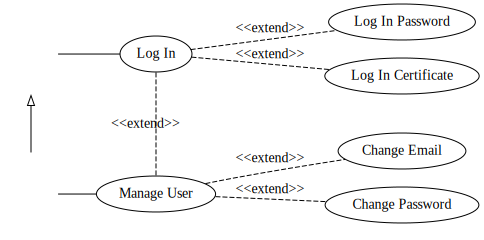
\includegraphics[scale=0.8]{use_case.png}
\caption{Use Case Diagram}
\label{fig:awesome_image}
\end{figure}

\begin{itemize}
    \item Two functional use cases:
    \begin{enumerate}
        \item \textbf{Read Display:} The user should be able to read the current temperature on the 7-segment display.
        \item \textbf{Set Mode:} The admin should be able to set the temperature mode. 
    \end{enumerate}
    \item One quality use case:
    \begin{enumerate}
        \item \textbf{Read Delta:} The delta value read by the user should be accurate within 0.1 degrees
    \end{enumerate}
\end{itemize}


\section*{Acceptance Test}
\begin{itemize}
    \item \textbf{Read Display:} 
        \begin{enumerate}
            \item Reset the system
            \item Enter temperature value 35
            \item Ensure that the 7-segment display shows 35
            \item Reset the system
            \item Enter temperature value 50
            \item Ensure that the 7-segment display shows 50
        \end{enumerate}

    \item \textbf{Set Mode:} 
        \begin{enumerate}
            \item Reset the system
            \item Set mode switch to 1 (negative values)
            \item Enter temperature value 40
            \item Ensure that the 7-segment shows -40
            \item Reset the system
            \item Set mode switch to 0 (positive values)
            \item Enter temperature value 40
            \item Ensure that the 7-segment shows 40
        \end{enumerate}

\end{itemize}

\section*{Implementation}
Modules supporting the above use cases:
        \begin{itemize}
            \item Temperature Input
            \item State Monitor
            \item Display Driver
            \item Display Output
        \end{itemize}
For this project a pure hardware solution was chosen due to the simplicity of the requirements. Incorporating software into this design would require some kind of softcore processor which would vastly increase the complexity.

\section*{Black Box Tests}
        \begin{itemize}
            \item \textbf{Temp input:} record the current temperature reading. Enter in a specific temperature on the switches and then press the .load. button. View the new current temperature reading as well as the last temperature reading and verify that they are correct.
            \item \textbf{State monitor:} enter in a temperature. Then enter in another temperature in a different state, verify that the new state is the correct state. Do this for each state transition.
            \item \textbf{Display driver:} Input a temperature, and state data. The output should be the corresponding display sequence for the Display Output module.
            \item \textbf{Display output:} Input decoded display data: temperature, state, alarm, delta. The output on the 7-segments should show the correct values
        \end{itemize}

\newpage
\section*{Sequence Diagram}

\begin{figure}[!htbp]
\centering
\includegraphics[scale=0.8]{seq_2.png}
\caption{Sequence Diagram}
\label{fig:seq_image}
\end{figure}

\section*{State Diagram}

\begin{figure}[!htbp]
\centering
\includegraphics[scale=0.8]{states.png}
\caption{Temperature State Diagram}
\label{fig:seq_image}
\end{figure}

\end{document}
